\ProvidesFile{rutitlepage.dtx}[2022/02/21 v3.0 Radboud University Titlepage]
\documentclass{ltxdoc}
\newcommand{\messagespace}{\text{$\mathcal{M}$}}
\newcommand{\messageinstance}{\text{$m$}}
\newcommand{\ciphertextspace}{\text{$\mathcal{C}$}}
\newcommand{\ciphertextinstance}{\text{$c$}}
\newcommand{\associateddataspace}{\text{$\mathcal{A}$}}
\newcommand{\associateddatainstance}{\text{$a$}}
\newcommand{\tagspace}{\text{$\mathcal{T}$}}
\newcommand{\taginstance}{\text{$t$}}
\newcommand{\keyspace}{\text{$\mathcal{K}$}}
\newcommand{\keyinstance}{\text{$k$}}
\newcommand{\noncespace}{\text{$\mathcal{N}$}}
\newcommand{\nonceinstance}{\text{$n$}}
\newcommand{\lockspace}{\text{$\mathcal{L}$}}
\newcommand{\lockinstance}{\text{$l$}}
\newcommand{\users}{\text{$N$}}
\newcommand{\user}{\text{$j$}}
\newcommand{\adversary}{\text{$A$}}
\newcommand{\sample}{\text{$\leftarrow$}}
\newcommand{\result}{\text{$\leftarrow$}}
\newcommand{\concatinate}{\text{$\|$}}

\newcommand{\advantage}[2]{\textbf{Adv}$_{\text{#1}}^{\text{#2}}$ }
\newcommand{\probabilityblock}[4]{\text{$|\text{Pr}[\text{#1}_{\text{#2}}^{\text{#3}}] - \text{Pr}[\text{#1}_{\text{#2}}^{\text{#4}}]|$}}

\newcommand{\pkc}{\text{Hybrid Encryption in a Multi-user Setting, revised}}
\newcommand{\gcrec}{\text{Generic Composition Reconsidered}}

\newcommand{\x}{\text{x}}
\usepackage{a4wide}
\usepackage{float}
\usepackage{graphicx}
\usepackage{array}
\usepackage[utf8]{inputenc}
\usepackage{rutitlepage}
\usepackage{fancyhdr}
\usepackage[style=ieee]{biblatex}
\usepackage[operators]{cryptocode}
\usepackage{amssymb}
\addbibresource{cryptobib/crypto.bib}
\GetFileInfo{rutitlepage.dtx}

\pagestyle{fancy}
\fancyhf{}
\lhead{Bachelor Thesis}
\rhead{Page \thepage}

\title{research proposal}
\author{stijnvandenput }
\date{20 May 2022}

\begin{document}
\maketitleru[
    layout=traditional,
    authors={Stijn Vandenput},
    authorstext={Author:},
    nextpagenr={-1},
    date={20/05/2022},
    institution={Radboud University},
    others={Supervisors:}{Martijn Stam\\Bart Mennink},
    course={Bachelor Thesis},
    title={TBD}]

\section*{Abstract}

\pagenumbering{roman}
\newpage
\tableofcontents

\newpage
\pagenumbering{arabic}

\section{Introduction}
Although symmetric and asymmetric cryptography are both subfields of cryptography, their research area's can be quite separated. This can lead to knowledge gaps between the two when work in asymmetric crypto uses constructions that are more common in symmetric crypto or the other way around. In this fashion, a paper by Giacon, Kiltz and Poettering \cite{PKC:GiaKilPoe18}, which we henceforth call \gkp{}, uses a construction that is very similar to Authenticated Encryption following the generic encrypt-then-MAC construction from Bellare and Namprempre \cite{AC:BelNam00}. This construction has since been revised in a paper by Namprempre, Rogaway and Thomas Shrimpton \cite{EC:NamRogShr14}, which we henceforth call \nrs{}. In this revision, a new set of constructions is given that be better applicable to common use cases. The aim of this thesis is to apply the knowledge from \nrs{} to the setting of \gkp{} and while doing so, create a new primitive for authenticated encryption suited for asymmetric settings.

\section{Preliminaries}
In this section we will explain several concepts important to the rest of our work, as well as some general notation.

\subsection{General Notation}
Strings are binary and bit-wise, the set of all strings is $\{0,1\}^\ast$. The length of x is written as $\abs{\text{x}}$, the concatenation of x and y as x \concatinate{} y, a being the result of b as a \result{} b and taking a random sampling from y and assigning it to x as x \sample{} y. We allow a single type of error message written as \invalid. \keyspace{} is a nonempty key space, \lockspace{} is a lock space, \noncespace{} is a nonce space, \messagespace{} is a message space and \associateddataspace{} is the associated-data space. \messagespace{} contain at least two strings, and if \messagespace{} or \associateddataspace{} contain a string of length x, it must contain all strings of length x. \users{} is the number of users.

\subsection{AE}

\subsection{PKE Schemes?}

\subsection{Nonces vs Locks (and different iv's)}

\subsection{Game Based Security Notions}

\subsection{Security Notions}
ind-\$/ind-lor/ind-cpa/ind-cca also note active and passive attackers

\subsection{Security Proofs}

\section{\nrs{} and \gkp{} in Detail}
In this section we explain the parts from \gkp{} and \nrs{} important to our work. Afterwards, a comparison is made between the two papers. Some notations will be different from the original papers for improved consistency. What are called tags in \gkp, we will call locks instead to avoid confusion with the output of mac functions and we call the output of the AMAC the tag instead of the ciphertext. The security notions from \nrs{} are converted to a game-based format using insights from (\textbf{todo add citation for Automated Analysis of Protocols that use Authenticated Encryption: How Subtle AEAD}) in order to better match the notation from \gkp{} and be more adaptable to a multi-user setting.

\subsection{\nrs}
Three generic ways to construct a authenticated encryption scheme are discussed in a paper written by Bellare and Namprempre \cite{AC:BelNam00}: encrypt-then-mac, encrypt-and-mac and mac-then-encrypt. In this paper, encrypt-then-mac is considered the only secure one when using probabilistic encryption as a building block. Within \nrs{} these constructions are generalized to using nonce- or iv-based encryption as a building block to create nonce-based authenticated encryption schemes, nAEs for short. We will look at the constructions using a nonce-based encryption, nE for short, and a PRF secure MAC function.

\subsubsection{Used Primitives}
\paragraph{nE}
A nonce-based encryption scheme is defined by triple $\mathit{\Pi}$ = $(\keyspace{},\text{E},\text{D})$. Deterministic encryption algorithm E takes three inputs $(\keyinstance,\nonceinstance,\messageinstance)$ and outputs a value \ciphertextinstance, the length of \ciphertextinstance{} only depends the length of \keyinstance, \nonceinstance{} and \messageinstance. If, and only if, $(\keyinstance,\nonceinstance,\messageinstance)$ is not in $\keyspace \times \noncespace \times \messagespace$, \ciphertextinstance{} will be \invalid. Decryption algorithm D takes three inputs $(\keyinstance,\nonceinstance,\ciphertextinstance)$ and outputs a value \messageinstance. Both E and D are required to satisfy correctness (if E$(\keyinstance,\nonceinstance,\messageinstance)$ $= \ciphertextinstance \neq \invalid$, then D$(\keyinstance,\nonceinstance,\ciphertextinstance)$ = \messageinstance) and tidiness (if D$(\keyinstance,\nonceinstance,\ciphertextinstance)$ $= \messageinstance \neq \invalid$, then E$(\keyinstance,\nonceinstance, \messageinstance)$ = \ciphertextinstance).

\paragraph{Security}
The security of a nE is defined as \advantage{$\mathit{\Pi}$,\adversary}{nE} = \probabilityblock{nE-IND\$}{\adversary}{0}{1}, where nE-IND\$ is in figure \ref{fig: nE-IND game}. In this game, set $U$ keeps track of all used nonces as the adversary is not allowed to repeat those.
\begin{figure}
    \centering
    \begin{pchstack}[boxed,center,space=0.5cm]
        \pseudocode[lnstart=-1,linenumbering,head={\textbf{Game} nE-IND\$$^{b}_{\adversary}$ }]{
            U \result \emptyset\\
            \keyinstance \sample \keyspace\\
            b' \result \adversary\\
            \pcreturn b'
        }
        \pseudocode[lnstart=4,linenumbering,head={\textbf{Oracle} Oenc$(\nonceinstance,\messageinstance)$}]{
            \pcif \nonceinstance \in U : \pcreturn \invalid\\
            U \result U \cup \{\nonceinstance\}\\
            \ciphertextinstance \result \text{E}(\keyinstance,\nonceinstance,\messageinstance)\\
            \pcif b = 1 \wedge \ciphertextinstance \neq \invalid: \\
            \t \ciphertextinstance \sample \{0,1\}^{\abs{\ciphertextinstance}}\\
            \pcreturn \ciphertextinstance
        }
    \end{pchstack}
    \caption{nE-IND\$ game, \adversary{} has access to oracle Oenc.}
    \label{fig: nE-IND game}
\end{figure}
    
\paragraph{MAC}
A MAC scheme is defined by algorithm F that takes a key \keyinstance{} in \keyspace{} and a string \messageinstance{} and outputs either a n-bit tag \taginstance{} or \invalid. The domain of F is the set X off al m such that F$(\keyinstance,\messageinstance)\neq \invalid$ is in X, this domain may not depend on \keyinstance.

\paragraph{Security}
The security of a MAC is defined as \advantage{F,\adversary}{MAC} = \probabilityblock{MAC-PRF}{\adversary}{0}{1}, where MAC-PRF is in figure \ref{fig: MAC-PRF}. In this game the set $U$ keeps track of the used messages to prevent trivial wins.
    \begin{figure}
        \centering
        \begin{pchstack}[boxed,center,space=0.5cm]
            \pseudocode[lnstart=-1,linenumbering,head={\textbf{Game} MAC-PRF$^{b}_{\adversary}$ }]{
                U \result \emptyset\\
                \keyinstance \sample \keyspace\\
                b' \result \adversary\\
                \pcreturn b'
            }
            \pseudocode[lnstart=3,linenumbering,head={\textbf{Oracle} Omac(\messageinstance)}]{
                \pcif \messageinstance \in U : \pcreturn \invalid\\
                U \result U \cup \{\messageinstance\}\\
                \taginstance \result \text{F}(\keyinstance,\messageinstance)\\
                \pcif b = 1 \wedge \taginstance \neq \invalid: \\
                \t \taginstance \sample \{0,1\}^{\abs{\taginstance}}\\
                \pcreturn \taginstance
            }
        \end{pchstack}
        \caption{MAC-PRF, \adversary{} has access to oracle Omac and $U$ is the set of used messages.}
        \label{fig: MAC-PRF}
    \end{figure}

\subsubsection{Nonce-Based Authenticated Encryption}
A nonce-based authenticated encryption scheme is defined by triple $\mathit{\Pi}$ = $(\keyspace{},\text{E},\text{D})$. Deterministic encryption algorithm E takes four inputs $(\keyinstance,\nonceinstance,\associateddatainstance,\messageinstance)$ and outputs a value \ciphertextinstance, the length of \ciphertextinstance{} only depends the length of \keyinstance, \nonceinstance, \associateddatainstance{} and \messageinstance. If, and only if, $(\keyinstance,\nonceinstance,\associateddatainstance,\messageinstance)$ is not in $\keyspace \times \noncespace \times \associateddataspace \times \messagespace$, \ciphertextinstance{} will be \invalid. Decryption algorithm D takes four inputs $(\keyinstance,\nonceinstance,\associateddatainstance,\ciphertextinstance)$ and outputs a value \messageinstance. both E and D are required to satisfy correctness (if E$(\keyinstance,\nonceinstance,\associateddatainstance,\messageinstance)$ $= \ciphertextinstance \neq \invalid$, then D$(\keyinstance,\nonceinstance,\associateddatainstance,\ciphertextinstance)$ = \messageinstance) and tidiness (if D$(\keyinstance,\nonceinstance,\associateddatainstance,\ciphertextinstance)$ $= \messageinstance \neq \invalid$, then E$(\keyinstance,\nonceinstance,\associateddatainstance,\messageinstance)$ = \ciphertextinstance). 

\paragraph{Security}
The security of a nAE is defined as \advantage{$\mathit{\Pi}$,\adversary}{nAE} = \probabilityblock{nAE-IND\$}{\adversary}{0}{1}, where nAE-IND\$ is in figure \ref{fig: nAE-IND game}. In this game, set $U$ keeps track of all used nonces as the adversary is not allowed to repeat those. Following the translation of IND\$ to a security game for AE from (\textbf{todo add citation for Automated Analysis of Protocols that use Authenticated Encryption: How Subtle AEAD}), \_ denotes a variable that is irrelevant and set $Q$ keeps tack of all query results in order to prevent trivial wins.
    \begin{figure}
        \centering
        \begin{pchstack}[boxed,center,space=0.5cm]
            \pseudocode[lnstart=-1,linenumbering,head={\textbf{Game} nAE-IND\$$^{b}_{\adversary}$ }]{
                U \result \emptyset\\
                Q \result \emptyset\\
                \keyinstance \sample \keyspace\\
                b' \result \adversary\\
                \pcreturn b'
            }
            \pseudocode[lnstart=5,linenumbering,head={\textbf{Oracle} Oenc$(\nonceinstance,\associateddatainstance,\messageinstance)$}]{
                \pcif \nonceinstance \in U : \pcreturn \invalid\\
                U \result U \cup \{\nonceinstance\}\\
                \pcif (\nonceinstance,\associateddatainstance,\messageinstance,\_) \in Q : \pcreturn \invalid\\
                \ciphertextinstance \result \text{E}(\keyinstance,\nonceinstance,\associateddatainstance,\messageinstance)\\
                \pcif b = 1 \wedge \ciphertextinstance \neq \invalid: \\
                \t \ciphertextinstance \sample \{0,1\}^{\abs{\ciphertextinstance}}\\
                Q \result Q \cup \{(\nonceinstance,\associateddatainstance,\messageinstance,\ciphertextinstance)\}\\
                \pcreturn \ciphertextinstance
            }
            \pseudocode[lnstart=13,linenumbering,head={\textbf{Oracle} Odec$(\nonceinstance,\associateddatainstance,\ciphertextinstance)$}]{
                \pcif b = 1 : \pcreturn \bot\\
                \pcif (\nonceinstance,\associateddatainstance,\_,\ciphertextinstance) \in Q : \pcreturn \invalid\\
                \messageinstance \result \text{D} (\keyinstance,\nonceinstance,\associateddatainstance,\ciphertextinstance)\\
                Q \result Q \cup \{(\nonceinstance,\associateddatainstance,\messageinstance,\ciphertextinstance)\}\\
                \pcreturn \messageinstance
            }
        \end{pchstack}
        \caption{nAE-IND\$ game, \adversary{} has access to oracles Oenc and Odec.}
        \label{fig: nAE-IND game}
    \end{figure}

\subsubsection{Construction}
A nAE scheme is constructed by several different schemes that combine the mac and nE into a nAE. We define the constructions secure as there is a tight reduction from breaking the nAE-security of the scheme to breaking the nE-security and the PRF security of the underlying primitives. Three different schemes, named N1, N2 and N3 were proven to be secure they can be viewed in figure 6 of \nrs{}. Noteworthy is that these relate to encrypt-and-mac, encrypt-then-mac,and mac-then-encrypt respectively, showing the general believe that encrypt-then-mac is the only safe construction does not transfer to this setting.

\subsection{\gkp}
In \gkp{}, the concept of augmentation using locks is discussed. The authors start by showing some data encapsulation mechanisms are vulnerable to a passive multi-instance distinguishing- and key recovery and how this can lead to problems when used in public key encryption. They define the augmented data encapsulation mechanisms, ADEM for short, that uses locks to negate these insecurities. Additionally, they show how a ADEM that is secure against passive attacks can be combined with a MAC that is augmented in a similar fashion, called a AMAC, to construct ADEM' that is safe against active attackers. This construction is similar to construction N2 from \nrs.

\subsubsection{Used Primitives}
In \gkp{}, \messagespace{} is not required to contain at least two strings, and to contain all strings of length x if it contains a string of length x. Additionally, \keyspace{} is required to be finite but not required to be non-empty. 
\paragraph{ADEM}
A ADEM scheme is defined by tuple $(\text{A.enc}, \text{A.dec})$. Deterministic algorithm A.enc takes a key \keyinstance{} in \keyspace{}, a lock \lockinstance{} in \lockspace{} and a message \messageinstance{} in \messagespace{} and outputs a ciphertext \ciphertextinstance{} in \ciphertextspace{}.  Deterministic algorithm A.dec takes a \keyinstance{} in \keyspace{}, a lock \lockinstance{} in \lockspace{} and a ciphertext \ciphertextinstance{} in \ciphertextspace{} and outputs a message \messageinstance{} in \messagespace{} or \invalid{} to indicate rejection. The correctness requirement is that for every combination of \keyinstance{}, \lockinstance{} and \messageinstance{} we have A.dec$(\keyinstance,\lockinstance,\text{A.enc}(\keyinstance,\lockinstance,\messageinstance))$ = \messageinstance. 

\paragraph{Security}
The security of a ADEM is defined as \advantage{ADEM,\adversary,\users}{l-ind-cpa} = \probabilityblock{L-IND-CPA}{\adversary,\users}{0}{1}, where L-IND-CPA is in figure \ref{fig: L-IND-CPA game}. Every user is only allowed one encryption query and locks may not repeat between users. Decryption queries are only allowed after the encryption. The corresponding game can be found in figure 9 from \gkp{}, note that this figure also included a decryption oracle the adversary is not allowed to use. (\textbf{Question: I do not really know if I should elaborate on how this translates to the game, as the game is based on the game of gkp})
\begin{figure}
    \centering
    \begin{pchstack}[boxed,center,space=0.5cm]
        \pseudocode[lnstart=-1,linenumbering,head={\textbf{Game} L-IND-CPA$^{b}_{\adversary,\users}$ }]{
        L \result \emptyset\\
        \pcfor \user \in [1..N]:\\
        \t \keyinstance_\user \sample \keyspace\\
        \t C_\user \result \emptyset\\
        b' \result \adversary\\
        \pcreturn b'
        }
        \pseudocode[lnstart=5,linenumbering,head={\textbf{Oracle} Oenc$(\user,\lockinstance,\messageinstance_0,\messageinstance_1)$}]{
            \pcif C_\user \neq \emptyset: \pcreturn \invalid\\
            \pcif \lockinstance \in L: \pcreturn \invalid\\
            L \result L \cup \{\lockinstance\}\\
            \lockinstance_\user \result \lockinstance\\
            \ciphertextinstance \result \text{A.enc}(\keyinstance_\user,\lockinstance_\user,\messageinstance_b)\\
            C_\user \result C_\user \cup \{\ciphertextinstance\}\\
            \pcreturn \ciphertextinstance
        }
    \end{pchstack}
    \caption{L-IND-CPA game, \adversary{} has access to oracle Oenc.}
    \label{fig: L-IND-CPA game}
\end{figure}

\paragraph{AMAC}
A AMAC scheme is defined by tuple $(\text{M.mac},\text{M.vrf})$. Deterministic algorithm M.mac takes a key \keyinstance{} in \keyspace{}, a lock \lockinstance{} in \lockspace{}, and a message \messageinstance{} in \messagespace{} and outputs a tag \taginstance{} in \tagspace{}. Deterministic algorithm M.vrf takes a key \keyinstance{} in \keyspace{}, a lock \lockinstance{} in \lockspace{}, a message \messageinstance{} in \messagespace{} and a ciphertext \taginstance{} in \tagspace{} and returns either \codetrue{} or \codefalse. The correctness requirement is that for every combination of \keyinstance{}, \lockinstance{} and \messageinstance{}, all corresponding \taginstance{} \result M.mac$(\keyinstance,\lockinstance,\messageinstance)$ gives M.vrf$(\keyinstance,\lockinstance,\messageinstance,\taginstance)$ = \codetrue. 

\paragraph{Security}
The security of a AMAC is defined as \advantage{AMAC,\adversary,\users}{L-MIOT-UF} = $\text{Pr}[\text{L-MIOT-UF}_{\adversary,\users} = 1]$, where L-MIOT-UF is in \ref{fig: L-MIOT-UF game}. Every user is only allowed one mac query and locks may not repeat between users. Verification queries are only allowed after the encryption. The corresponding game can be found in figure 15 of \gkp{}.
\begin{figure}
    \centering
    \begin{pchstack}[boxed,center,space=0.5cm]
        \pseudocode[lnstart=-1,linenumbering,head={\textbf{Game} L-MIOT-UF$_{\adversary,\users}$ }]{
        \text{forged} \result 0\\
        L \result \emptyset\\
        \pcfor \user \in [1..N]:\\
        \t \keyinstance_\user \sample \keyspace\\
        \t T_\user \result \emptyset\\
        \textbf{run } \adversary\\
        \pcreturn \text{forged}
        }
        \pseudocode[lnstart=6,linenumbering,head={\textbf{Oracle} Omac$(\user,\lockinstance,\messageinstance)$}]{
            \pcif T_\user \neq \emptyset: \pcreturn \invalid\\
            \pcif \lockinstance \in L: \pcreturn \invalid\\
            L \result L \cup \{\lockinstance\}\\
            \lockinstance_\user \result \lockinstance\\
            \taginstance \result \text{M.mac}(\keyinstance_\user,\lockinstance_\user,\messageinstance)\\
            T_\user \result T_\user \cup \{(\messageinstance,\taginstance)\}\\
            \pcreturn \taginstance
        }
        \pseudocode[lnstart=13,linenumbering,head={\textbf{Oracle} Ovrf$(\user,\messageinstance,\taginstance)$}]{
            \pcif T_\user = \emptyset: \pcreturn \invalid\\
            \pcif (\messageinstance,\taginstance) \in T_\user: \pcreturn \invalid\\
            \pcif \text{M.vrf}(\keyinstance_\user,\lockinstance_\user,\messageinstance,\taginstance): \\
            \t \text{forged} \result 1\\
            \t \pcreturn \codetrue\\
            \pcelse : \pcreturn \codefalse
        }
    \end{pchstack}
    \caption{L-MIOT-UF game, \adversary{} has access to oracles Omac and Ovrf and the locks in line 11 and 16 are the same.}
    \label{fig: L-MIOT-UF game}
\end{figure}

\subsubsection{ADEM'}
A ADEM' scheme is defined by tuple $(\text{A.enc'}, \text{A.dec'})$. Deterministic algorithm A.enc' takes a key \keyinstance{} in \keyspace{}, a lock \lockinstance{} in \lockspace{} and a message \messageinstance{} in \messagespace{} and outputs a ciphertext \ciphertextinstance{} in \ciphertextspace{}. Deterministic algorithm A.dec' takes a \keyinstance{} in \keyspace{}, a lock \lockinstance{} in \lockspace{} and a ciphertext \ciphertextinstance{} in \ciphertextspace{} and outputs a message \messageinstance{} in \messagespace{} or \invalid{} to indicate rejection. The correctness requirement is that for every combination of \keyinstance{}, \lockinstance{} and \messageinstance{} we have A.dec'$(\keyinstance,\lockinstance,\text{A.enc'}(\keyinstance,\lockinstance,\messageinstance))$ = \messageinstance.

\paragraph{Security}
The security of a ADEM' is defined as \advantage{ADEM',\adversary,\users}{l-ind-cca} = \probabilityblock{L-IND-CCA}{\adversary,\users}{0}{1}, where L-IND-CCA is in \ref{fig: L-IND-CCA game}. Every user is only allowed one encryption query and locks may not repeat between users. Decryption queries are only allowed after the encryption. The corresponding game can be found in figure 9 of \gkp{}.
\begin{figure}
    \centering
    \begin{pchstack}[boxed,center,space=0.5cm]
        \pseudocode[lnstart=-1,linenumbering,head={\textbf{Game} L-IND-CCA$^{b}_{\adversary,\users}$ }]{
        L \result \emptyset\\
        \pcfor \user \in [1..N]:\\
        \t \keyinstance_\user \sample \keyspace\\
        \t C_\user \result \emptyset\\
        b' \result \adversary\\
        \pcreturn b'
        }
        \pseudocode[lnstart=5,linenumbering,head={\textbf{Oracle} Oenc$(\user,\lockinstance,\messageinstance_0,\messageinstance_1)$}]{
            \pcif C_\user \neq \emptyset: \pcreturn \invalid\\
            \pcif \lockinstance \in L: \pcreturn \invalid\\
            L \result L \cup \{\lockinstance\}\\
            \lockinstance_\user \result \lockinstance\\
            \ciphertextinstance \result \text{A.enc'}(\keyinstance_\user,\lockinstance_\user,\messageinstance_b)\\
            C_\user \result C_\user \cup \{\ciphertextinstance\}\\
            \pcreturn \ciphertextinstance
        }
        \pseudocode[lnstart=12,linenumbering,head={\textbf{Oracle} Odec(\user,\ciphertextinstance)}]{
            \pcif C_\user = \emptyset: \pcreturn \invalid\\
            \pcif \ciphertextinstance \in C_\user: \pcreturn \invalid\\
            \messageinstance \result \text{A.dec'}(\keyinstance_\user,\lockinstance_\user,\ciphertextinstance)\\
            \pcreturn \messageinstance
        }
    \end{pchstack}
    \caption{L-IND-CCA game, \adversary{} has access to oracles Oenc and Odec and the locks in line 10 and 15 are the same.}
    \label{fig: L-IND-CCA game}
\end{figure}

\subsubsection{Construction}
The ADEM' scheme considered is made by creating A.enc' and A.dec' calls using the calls the primitives provide us as seen in figure \ref{fig: A.enc' and A.dec' calls}.
\begin{figure}
    \centering
    \begin{pchstack}[boxed,center,space=0.5cm]
        \pseudocode[lnstart=-1,linenumbering,head={\textbf{Proc} A.enc'$(\keyinstance,\lockinstance,\messageinstance)$}]{
        (\keyinstance_{dem},\keyinstance_{mac}) \result \keyinstance\\
        \ciphertextinstance' \result \text{A.enc}(\keyinstance_{dem},\lockinstance,\messageinstance)\\
        \taginstance \result \text{M.mac}(\keyinstance_{mac},\lockinstance,\ciphertextinstance')\\
        \ciphertextinstance \result (\ciphertextinstance',\taginstance)\\
        \pcreturn \ciphertextinstance
        }
        \pseudocode[lnstart=4,linenumbering,head={\textbf{Proc} A.dec'$(\keyinstance,\lockinstance,\ciphertextinstance)$}]{
            (\keyinstance_{dem},\keyinstance_{mac}) \result \keyinstance\\
            (\ciphertextinstance',\taginstance) \result \ciphertextinstance\\
            \pcif \text{M.vrf}(\keyinstance_{mac},\lockinstance,\ciphertextinstance',\taginstance):\\
            \t \messageinstance \result \text{A.dec}(\keyinstance_{dem},\lockinstance,\ciphertextinstance')\\
            \t \pcreturn \messageinstance\\
            \pcelse : \pcreturn \invalid
        }
    \end{pchstack}
    \caption{A.enc' and A.dec' calls, The corresponding calls can be found in figure 16 of \gkp{}.}
    \label{fig: A.enc' and A.dec' calls}
\end{figure}
\noindent The construction is deemed secure as for any \users{} and a \adversary{} that makes $Q_d$ many Odec queries, the exist $B$ and $C$ such that \advantage{ADEM',$A$,\users}{l-ind-cca} $\leq$ 2\advantage{AMAC,$B$,\users}{l-miot-uf} + \advantage{ADAM,$C$,\users}{l-ind-cpa} holds. Where the running time of $B$ is at most that of $A$ plus the time required to run \users-many ADEM encapsulations and $Q_d$-many ADEM decapsulations and the running time of $C$ is the same as the running time of $A$. Additionally, $B$ poses at most $Q_d$-many Ovrf queries, and $C$ poses no Odec query.

\subsection{Comparison of \gkp{} and \nrs}
In this section we will highlight the important differences between \gkp{} and \nrs{}. (\textbf{Question: I feel like this section is very factual right now, while it might also be worthwhile to elaborate on some things a bit more.})

\paragraph{Setting}
\nrs{} is written is single-user, multiple-use key setting while \gkp{} is written is a multi-user, single-use key setting. As a result, \gkp{} uses locks while \nrs{} uses nonces. (\textbf{Question: is it necessary to elaborate on how these settings lead to lock, or nonce usage, or would it suffice to explain this in section 2.4}).

\paragraph{Aim}
While \nrs{} is aimed at generalizing the AE constructions, \gkp{} is aimed aimed at finding a single construction that is safe when used in public key encryption. Most notably, this results in \nrs{} evaluating 20 possible constructions while \gkp{} evaluates one. Additionally, the constructions from \nrs{} are able to use AD while the construction form \gkp{} cannot.

\paragraph{Security Notion}
The security notions of \nrs{} are written in a IND\$ fashion while the security notions of \gkp{} are written in a lor fashion. In other words, \nrs{} requires the valid ciphertext to be indistinguishable from random strings, \gkp{} only requires them to be indistinguishable from each other. As a result, the MAC primitives of the two papers have different security requirements. In \nrs{}, the tag is required to be indistinguishable from a random string while in \gkp{} the tag is only required to be unforgeable.

\section{Defining the New Primitive}
In this section we will discuss a new security primitive, the lock-based one time use Authenticated Encryption scheme, loAE scheme for short. As the name suggests, this primitive is used in a setting where a key is used only once to encrypt and authenticate a single message. We uses locks instead of nonces, as you will never have to decrypt messages with multiple nonces for a single user. Below, we discuss the notation of the loAE.

\subsection{loAE}
A loAE scheme is defined by tuple $(\text{AE.enc},\text{AE.dec})$. Deterministic algorithm AE.enc takes three inputs $(\keyinstance,\lockinstance,\messageinstance)$ and outputs a value \ciphertextinstance, the length of \ciphertextinstance{} only depends on the length of \keyinstance, \lockinstance{} and \messageinstance. If, and only if $(\keyinstance,\lockinstance,\messageinstance)$ is not in $\keyspace \times \lockspace \times \messagespace$, \ciphertextinstance{} will be \invalid. Deterministic algorithm AE.dec takes three inputs $(\keyinstance,n,\ciphertextinstance)$ and outputs a value \messageinstance. Both AE.enc and EA.dec are required to satisfy correctness (if AE.enc$(\keyinstance,\lockinstance,\messageinstance)$ $= \ciphertextinstance \neq \invalid$, then AE.dec$(\keyinstance,\lockinstance,\ciphertextinstance)$ = \messageinstance) and tidiness (if AE.dec$(\keyinstance,\lockinstance,\ciphertextinstance)$ $= \messageinstance \neq \invalid$, then AE.enc$(\keyinstance,\lockinstance,\messageinstance)$ = \ciphertextinstance).

\subsection{Security Model}
To define the security, we use a ind\$ security notion instead of left-or-right one as, in our setting, ind\$ is the stronger security notion. (\textbf{Question: is it necessary to elaborate on how this here, or would it suffice to explain this in section 2.6}) We use a function that always returns \invalid{} on decryption calls to ensure the adversary can not guess which ciphertexts would be valid ciphertexts. To match our setting, the user is only allowed one encryption query, locks may not repeat between users and decryption queries are only allowed after the encryption.The security is defined as \advantage{\adversary,\users}{loAE} = \probabilityblock{loAE-IND\$}{\adversary,\users}{0}{1}, where loAE-IND\$ is in figure \ref{fig: nAE-IND game}.
\begin{figure}
    \begin{pchstack}[boxed,center,space=0.5cm]
        \pseudocode[lnstart=-1,linenumbering,head={\textbf{Game} loAE-IND\$$^{b}_{\adversary,\users}$ }]{
        L \result \emptyset\\
        \pcfor \user \in [1..N]:\\
        \t \keyinstance_\user \sample \keyspace\\
        \t C_\user \result \invalid\\
        b' \result \adversary\\
        \pcreturn b'
        }
        \pseudocode[lnstart=5,linenumbering,head={\textbf{Oracle} Oenc$(\user,\lockinstance,\messageinstance)$}]{
            \pcif C_\user \neq \invalid: \pcreturn \invalid\\
            \pcif \lockinstance \in L: \pcreturn \invalid\\
            L \result L \cup \{\lockinstance\}\\
            \lockinstance_\user \result \lockinstance\\
            \ciphertextinstance \result \text{AE.enc}(\keyinstance_\user,\lockinstance_\user,\messageinstance)\\
            \pcif b = 1 \wedge \ciphertextinstance \neq \invalid: \\
            \t \ciphertextinstance \sample \{0,1\}^{\abs{\ciphertextinstance}}\\
            C_\user \result \ciphertextinstance\\
            \pcreturn \ciphertextinstance
        }
        \pseudocode[lnstart=14,linenumbering,head={\textbf{Oracle} Odec$(\user,\ciphertextinstance)$}]{
            \pcif C_\user = \invalid: \pcreturn \invalid\\
            \pcif \ciphertextinstance = C_\user: \pcreturn \invalid\\
            \messageinstance \result \text{AE.dec}(\keyinstance_\user,\lockinstance_\user,\ciphertextinstance)\\
            \pcif b = 1 : \messageinstance = \bot\\
            \pcreturn \messageinstance
        }
    \end{pchstack}
    \caption{loAE-IND\$ game, adversary{} has access to oracles Oenc and Odec.}
    \label{fig: loAE-IND game}
\end{figure}

\subsection{Explanation of the Security Model}
In this subsection we will discuss the security game loAE-IND\$ line by line.\\
\begin{tabular}{|m{13,5cm}|}
\hline Draft:\\
\textit{line 0:} We start by initializing the set of all used locks to the empty set.
\textit{line 1:} Next we loop over each user to initialize them.
\textit{line 2:} For each user, we sample a uniformly random key from the key space and assign it to that user-key.
\textit{line 3:} for each user, we initialize the user-ciphertext to be undefined. We do not use set notation for this as done in \gkp{}, as we can never have multiple ciphertexts related to one user.
\textit{line 4:} After initializing all users, we run the algorithm of the adversary and safe the output.
\textit{line 5:} We end by returning this output.
\textit{line 6:} We do not allow multiple encryptions per user. Therefore, if the ciphertexts is defined we return \invalid.
\textit{line 7:} Locks are not allowed to repeat, if the lock is in the set of used sets we return \invalid.
\textit{line 8:} If these checks pass, we start the encryption by adding the lock to the sets of used locks
\textit{line 9:} We bind the lock to the user-lock.
\textit{line 10:} We encrypt the message using the user-key and the user-lock.
\textit{line 11:} The random function should return \invalid{} whenever AE returns \invalid{}. Therefore the random function is only called if b = 1 and AE does not return \invalid.
\textit{line 12:} The random function samples a string with the uniformly at random from the set of all strings with the length of the ciphertext. \textbf{(todo: add part about ideal vs attainable)}
\textit{line 13:} The computed ciphertext is bound to the user-ciphertext. \textbf{(todo: add part about the fact that this might be \invalid)}
\textit{line 14:} Return the ciphertext.
\textit{line 15:} If the user-ciphertext is not defined, decryption is not allowed and we return \invalid.
\textit{line 16:} If the input ciphertext of Odec is allowed to be the same as the user-ciphertext, then it is trivial to distinguish as in this case the ideal words will return \invalid{} while the real world does not. For this reason the real world should return \invalid{} as well.
\textit{line 17:} If these checks pass, we decrypt the ciphertext.
\textit{line 18:} The ideal world always returns \invalid{}.
\textit{line 19:} We return the decrypted message.\\
\hline
\end{tabular}

\section{Constructions}
In this section we discuss how we can construct a safe loAE. Similarly to \gkp{} and \nrs{} we will look at constructions combining a deterministic encryption primitive and mac primitive. First write down the definitions of these two primitives, then we will look at how we can combine the two and which security bounds we can expect. Lastly we compare our choices with existing alternatives.

\subsection{Used Primitives}
\paragraph{loE}
A lock-based one time use encryption scheme, loE for short, is defined by tuple $(\text{E.enc},\text{E.dec})$. Deterministic algorithm E.enc takes three inputs $(\keyinstance,\lockinstance,\messageinstance)$ and outputs a value \ciphertextinstance, the length of \ciphertextinstance{} only depends on the length of \keyinstance, \lockinstance{} and \messageinstance. If, and only if, $(\keyinstance,\lockinstance,\messageinstance)$ is not in $\keyspace \times \lockspace \times \messagespace$, \ciphertextinstance{} will be \invalid. Deterministic algorithm E.dec takes three inputs $(\keyinstance,\lockinstance,\ciphertextinstance)$ and outputs a value \messageinstance. Both E.enc and E.dec are required to satisfy correctness (if E.enc$(\keyinstance,\lockinstance,\messageinstance)$ $= \ciphertextinstance \neq \invalid$, then E.dec$(\keyinstance,\lockinstance,\ciphertextinstance)$ = \messageinstance) and tidiness (if E.dec$(\keyinstance,\lockinstance,\ciphertextinstance)$ $= \messageinstance \neq \invalid$, then E.enc$(\keyinstance,\lockinstance,\messageinstance)$ = \ciphertextinstance). 

\paragraph{Security}
The security of a loE is defined as \advantage{\adversary,\users}{loE} = \probabilityblock{loE-IND\$}{\adversary,\users}{0}{1}, where loE-IND\$ is in figure \ref{fig: loE-IND game}. The user is only allowed one encryption query and locks may not repeat between users. Decryption queries are only allowed after the encryption.
    \begin{figure}
        \begin{pchstack}[boxed,center,space=0.5cm]
            \pseudocode[lnstart=-1,linenumbering,head={\textbf{Game} loE-IND\$$^{b}_{\adversary,\users}$ }]{
            L \result \emptyset\\
            \pcfor \user \in [1..\users]:\\
            \t \keyinstance{}_\user \sample \keyspace\\
            \t C_\user \result \invalid\\
            b' \result \adversary\\
            \pcreturn b'
            }
            \pseudocode[lnstart=5,linenumbering,head={\textbf{Oracle} Oenc$(\user,\lockinstance,\messageinstance)$}]{
                \pcif C_\user \neq \invalid: \pcreturn \invalid\\
                \pcif \lockinstance \in L: \pcreturn \invalid\\
                L \result L \cup \{\lockinstance\}\\
                \lockinstance{}_\user \result \lockinstance\\
                \ciphertextinstance \result \text{E.enc}(\keyinstance{}_\user,\lockinstance{}_\user,\messageinstance)\\
                \pcif b = 1 \wedge \ciphertextinstance \neq \invalid: \\
                \t \ciphertextinstance \sample \{0,1\}^{\abs{\ciphertextinstance}}\\
                C_\user \result \ciphertextinstance\\
                \pcreturn \ciphertextinstance
            }
        \end{pchstack}
    \caption{loE-IND\$ game, \adversary has access to oracle Oenc.}
    \label{fig: loE-IND game}
    \end{figure}
    
\paragraph{loMAC}
A lock-based one time use MAC is a deterministic algorithm M.mac that takes a fixed length \keyinstance{} in \keyspace{}, a fixed length \lockinstance{} in \lockspace{} and a variable length message \messageinstance{} in \messagespace{} and outputs either a n-bit length string we call tag \taginstance, or \invalid. If, and only if, $(\keyinstance,\lockinstance,\messageinstance)$ is not in $\keyspace \times \lockspace \times \messagespace$, \taginstance{} will be \invalid. 

\paragraph{Security}
The security of a PRF-MAC is defined as \advantage{F,\adversary,\users}{loMAC} = \probabilityblock{loMAC-PRF}{\adversary,\users}{0}{1}, where loMAC-PRF is in figure \ref{fig: loMAC-PRF game}. The user is only allowed one mac query and locks may not repeat between users. Verification queries are only allowed after the encryption.
    \begin{figure}
        \centering
        \begin{pchstack}[boxed,center,space=0.5cm]
            \pseudocode[lnstart=-1,linenumbering,head={\textbf{Game} loMAC-PRF$^{b}_{\adversary,\users}$ }]{
                L \result \emptyset\\
                \pcfor \user \in [1..N]:\\
                \t \keyinstance_\user \sample \keyspace\\
                \t T_\user \result \invalid\\
                b' \result A\\
                \pcreturn b'
            }
            \pseudocode[lnstart=5,linenumbering,head={\textbf{Oracle} Omac$(\user,\lockinstance,\messageinstance)$}]{
                \pcif T_\user \neq \invalid: \pcreturn \invalid\\
                \pcif \lockinstance \in L: \pcreturn \invalid\\
                L \result L \cup \{\lockinstance\}\\
                \lockinstance_\user \result \lockinstance\\
                \taginstance \leftarrow \text{M.mac}(\keyinstance_\user,\lockinstance_\user,\messageinstance)\\
                \pcif b = 1 \wedge \taginstance \neq \invalid: \\
                \t \taginstance \sample \{0,1\}^{\abs{\taginstance}}\\
                T_\user \result (\messageinstance,\taginstance)\\
                \pcreturn \taginstance
            }
            \pseudocode[lnstart=14,linenumbering,head={\textbf{Oracle} Ovrf$(\user,\messageinstance,\taginstance)$}]{
                \pcif T_\user = \invalid: \pcreturn \invalid\\
                \pcif (\messageinstance,\taginstance) = T_\user : \pcreturn \invalid \\
                \pcif b = 1 : \pcreturn \codefalse\\
                \taginstance' \leftarrow \text{M.mac}(\keyinstance_\user,\lockinstance_\user,\messageinstance)\\
                \pcif \taginstance = \taginstance' \\
                \t \pcreturn \codetrue\\
                \pcreturn \codefalse
            }
        \end{pchstack}
        \caption{loMAC-PRF game, \adversary{} has access to oracle Omac.}
        \label{fig: loMAC-PRF game}
    \end{figure}

\subsection{Construction}
Following \nrs{}, three ways to construct this loAE are of interest, namely the ones following from the N1, N2 and N3 scheme. The schemes, adjusted to our setting, are in figure \ref{fig: N schemes}. \nrs{} considers 17 more schemes but as no one of them has proven to be secure we will not consider those. The AE.enc and AE.dec calls corresponding to N1, N2 and N3 are in figure \ref{fig: N1 calls}, \ref{fig: N2 calls} and \ref{fig: N3 calls} respectively.
\begin{figure}
    \centering
    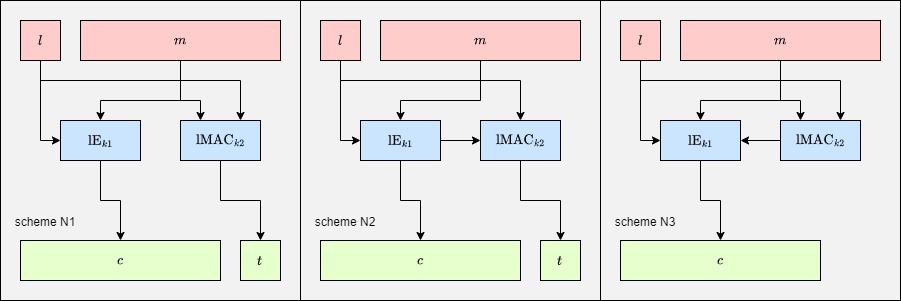
\includegraphics[scale = 0.4]{images/N-schemes.png}
\caption{Adjusted N schemes from \nrs}
\label{fig: N schemes}
\end{figure}

\begin{figure}
    \begin{pchstack}[boxed,center,space=0.5cm]
        \pseudocode[lnstart=-1,linenumbering,head={AE.enc$(\keyinstance,\lockinstance,\messageinstance)$}]{
            (\keyinstance{}1,\keyinstance{}2) \result \keyinstance \\
            \ciphertextinstance' \result \text{E.enc}(\keyinstance{}1,\lockinstance,\messageinstance) \\
            \taginstance \result \text{M.mac}(\keyinstance{}2,\lockinstance,\messageinstance) \\
            \ciphertextinstance \result (\ciphertextinstance',\taginstance)\\
            \pcreturn \ciphertextinstance
        }
        \pseudocode[lnstart=4,linenumbering,head={AE.dec$(\keyinstance,\lockinstance,\ciphertextinstance)$}]{
            (\keyinstance{}1,\keyinstance{}2) \result \keyinstance \\
            (\ciphertextinstance',\taginstance) \result \ciphertextinstance \\
            \messageinstance \result \text{E.dec}(\keyinstance{}1,\lockinstance,\ciphertextinstance') \\
            \taginstance' \result \text{M.mac}(\keyinstance{}2,\lockinstance,\messageinstance) \\
            \pcif \taginstance = \taginstance' : \pcreturn \messageinstance \\
            \pcelse : \pcreturn \invalid
        }
    \end{pchstack}
\caption{Calls based on N1}
\label{fig: N1 calls}
\end{figure}

\begin{figure}
    \begin{pchstack}[boxed,center,space=0.5cm]
        \pseudocode[lnstart=-1,linenumbering,head={AE.enc$(\keyinstance,\lockinstance,\messageinstance)$}]{
            (\keyinstance{}1,\keyinstance{}2) \result \keyinstance\\
            \ciphertextinstance' \result \text{E.enc}(\keyinstance{}1,\lockinstance,\messageinstance)\\
            \taginstance \result \text{M.mac}(\keyinstance{}2,\lockinstance,\ciphertextinstance')\\
            \ciphertextinstance \result (\ciphertextinstance',\taginstance)\\
            \pcreturn \ciphertextinstance
        }
        \pseudocode[lnstart=4,linenumbering,head={AE.dec$(\keyinstance,\lockinstance,\ciphertextinstance)$}]{
            (\keyinstance{}1,\keyinstance{}2) \result \keyinstance\\
            (\ciphertextinstance',\taginstance) \result \ciphertextinstance\\
            \messageinstance \result \text{E.dec}(\keyinstance{}1,\lockinstance,\ciphertextinstance')\\
            \taginstance' \result \text{M.mac}(\keyinstance{}2,\lockinstance,\ciphertextinstance')\\
            \pcif \taginstance = \taginstance' : \pcreturn \messageinstance \\
            \pcelse : \pcreturn \invalid
        }
    \end{pchstack}
\caption{Calls based on N2}
\label{fig: N2 calls}
\end{figure}

\begin{figure}
    \begin{pchstack}[boxed,center,space=0.5cm]
        \pseudocode[lnstart=-1,linenumbering,head={AE.enc$(\keyinstance,\lockinstance,\messageinstance)$}]{
            (\keyinstance{}1,\keyinstance{}2) \result \keyinstance\\
            \taginstance \result \text{M.mac}(\keyinstance{}2,\lockinstance,\messageinstance)\\
            \messageinstance' \result \messageinstance \concatinate \taginstance\\
            \ciphertextinstance \result E.enc(\keyinstance{}1,\lockinstance,\messageinstance')\\
            \pcreturn \ciphertextinstance
        }
        \pseudocode[lnstart=4,linenumbering,head={AE.dec$(\keyinstance,\lockinstance,\ciphertextinstance)$}]{
            (\keyinstance{}1,\keyinstance{}2) \result \keyinstance\\
            \messageinstance' \result \text{E.dec}(\keyinstance{}1,\lockinstance,\ciphertextinstance)\\
            (\messageinstance,\taginstance) \result \messageinstance'\\
            \taginstance' \result \text{M.mac}(\keyinstance{}2,\lockinstance,\messageinstance)\\
            \pcif \taginstance = \taginstance' : \pcreturn \messageinstance \\
            \pcelse : \pcreturn \invalid
        }
    \end{pchstack}
\caption{Calls based on N3}
\label{fig: N3 calls}
\end{figure}

\subsection{Security Bounds}
We define the constructions secure if there is a tight reduction from breaking the loAE-security of the scheme to breaking the loE-security and the loMAC security of the underlying primitives.

\subsection{Comparison with Existing Alternatives}

\section{Use Cases}
should consist of:
\begin{itemize}
	\item possible use cases
\end{itemize}
\subsection{PKE Schemes}

\section{Related Work}
\textbf{Location not final yet}

\section{Conclusion}

\newpage
\printbibliography[heading=bibintoc,title={References}]
\section{Appendix A}
(\textbf{todo: elaborate more on this table})\\
Below is a table which highlights the differences in notation between \gkp{} and \nrs, as well as give the notation I will be using.\\
\begin{tabular}[H]{|c | c | c | c | m{4,5cm}|}
    \hline
    Name   &   \gkp   &   \nrs   &   my notation & rough meaning \\[0.5 ex]
    \hline
    \hline
    message   &   $m$   &   $M$   &   \messageinstance &  message the user sends \\
    \hline
    ciphertext space   &   $\mathcal{C}$   &   -   &   \ciphertextspace & set of all possible ciphertext options \\
    \hline
    ciphertext   &   $c$   &   $C$   &   \ciphertextinstance & encrypted message \\
    \hline
    associated data   &   -   &   $A$   &   \associateddatainstance & data you want to authenticate but not encrypt \\
    \hline
    tag space   &   $\mathcal{C}$   &   -   &   \tagspace & set off all possible tag options \\
    \hline
    tag   &   $c$   &   $T$   &   \taginstance & output of mac function \\
    \hline
    key   &   $k$   &   $K$   &   \keyinstance   & user key \\
    \hline
    nonce space   &   -   &   $\mathcal{N}$   &   \noncespace & set of all nonce options \\
    \hline
    nonce   &   -   &   $n$   &   \nonceinstance & number only used once \\
    \hline
    lock space   &   $\mathcal{T}$   &   -   &   \lockspace & set of all possible lock options \\
    \hline
    lock   &   $t$   &   -   &   \lockinstance & nonce that is bound to the user \\
    \hline
    adversary   &   A   &   $\mathcal{A}$   &   \adversary & the bad guy \\
    \hline
    random sampling   &   $\xleftarrow{\$}$    &   $\twoheadleftarrow$   &   \sample & get a random ellermetn form the set \\
    \hline
    result of randomized function   &   $\xleftarrow{\$}$   &   -   &   \result & get the result of a randomized function with given inputs \\
    \hline
    %Name   &   \gkp   &   \GCrec   &   my notation & rough meaning \\
    %\hline
\end{tabular}

\end{document}

\NeedsTeXFormat{LaTeX2e}
\ProvidesPackage{rutitlepage}[2022/02/21 Mart Lubbers]
\RequirePackage{geometry,graphicx,ifpdf,keyval,iflang}
\def\@rutitleauthors{\@author}
\def\@rutitleauthorstext{Aut\IfLanguageName{dutch}{eu}{ho}r:}
\def\@rutitledate{\@date}
\def\@rutitleinst{Radboud Universit\IfLanguageName{dutch}{eit}{y} Nijmegen}
\def\@rutitletitle{\@title}
\def\@rutitlelayout{twentytwo}
\newif\if@rutitlecolour\@rutitlecolourfalse
\define@key{maketitleru}{authors}{\def\@rutitleauthors{#1}}
\define@key{maketitleru}{authorstext}{\def\@rutitleauthorstext{#1}}
\define@key{maketitleru}{colour}[true]{\@rutitlecolourtrue}
\define@key{maketitleru}{course}{\def\@rutitlecourse{#1}}
\define@key{maketitleru}{date}{\def\@rutitledate{#1}}
\define@key{maketitleru}{institution}{\def\@rutitleinst{#1}}
\define@key{maketitleru}{layout}{\def\@rutitlelayout{#1}}
\define@key{maketitleru}{nextpagenr}{\def\@rutitlenextpagenr{#1}}
\define@key{maketitleru}{others}{\def\@rutitleothers{#1}}
\define@key{maketitleru}{subtitle}{\def\@rutitlesubtitle{#1}}
\define@key{maketitleru}{title}{\def\@rutitletitle{#1}}
\newcommand*{\rutitlepage@printothers}[2]{\textit{#1}\\#2}
\newcommand*{\rutitlepage@sepothers}{\\[\baselineskip]}
\newcommand*{\rutitlepage@others}[2]{%
	\rutitlepage@printothers{#1}{#2}%
	\kernel@ifnextchar,{\rutitlepage@sepothers\rutitlepage@otherslist@}\relax}
\newcommand*{\rutitlepage@otherslist}[1]{%
	\expandafter\rutitlepage@others#1}
\def\rutitlepage@otherslist@,#1{\rutitlepage@otherslist{{#1}}}
\newcommand{\rutitle@layout@twentytwo}[0]{
	\newgeometry{left=25mm,top=25mm,right=15mm,bottom=10mm,hmarginratio=1:1}
	\begin{titlepage}%
		\null\vfill%
		\parindent0pt
		\ifdefined\@rutitlecourse\textsc{\LARGE\@rutitlecourse}\\[1.5cm]\fi
		{\Huge\bfseries\@rutitletitle}%
		\ifdefined\@rutitlesubtitle{\\[2\baselineskip]\large\itshape\@rutitlesubtitle\/}\fi\\[4\baselineskip]
		{\Large\scshape\@rutitleauthors}\\[\baselineskip]
		{\large\@rutitledate}
		\vfill

		\ifdefined\@rutitleothers\rutitlepage@otherslist\@rutitleothers\fi
		\vfill

		\hfill
		\ifpdf\includegraphics[width=80mm]{rutitlepage-logo-\IfLanguageName{dutch}{nl-}{}\if@rutitlecolour cmyk\else bw\fi.pdf}\\
		\else\includegraphics[width=80mm]{rutitlepage-logo-\IfLanguageName{dutch}{nl-}{}\if@rutitlecolour cmyk\else bw\fi.eps}\\
		\fi
	\end{titlepage}
	\restoregeometry%
}
\newcommand{\rutitle@layout@seventeen}[0]{
	\newgeometry{left=25mm,top=25mm,right=15mm,bottom=10mm,hmarginratio=1:1}
	\begin{titlepage}%
		\null\vfill%
		\parindent0pt
		{\Huge\bfseries\@rutitletitle}%
		\ifdefined\@rutitlesubtitle{\\[2\baselineskip]\large\itshape\@rutitlesubtitle\/}\fi\\[4\baselineskip]
		{\Large\scshape\@rutitleauthors}\\[\baselineskip]
		{\large\@rutitledate}
		\vfill

		\ifdefined\@rutitleothers\rutitlepage@otherslist\@rutitleothers\fi
		\vfill

		\hfill
		\ifpdf\includegraphics[width=80mm]{rutitlepage-logo-\IfLanguageName{dutch}{nl-}{}\if@rutitlecolour cmyk\else bw\fi.pdf}\\
		\else\includegraphics[width=80mm]{rutitlepage-logo-\IfLanguageName{dutch}{nl-}{}\if@rutitlecolour cmyk\else bw\fi.eps}\\
		\fi
	\end{titlepage}
	\restoregeometry%
}
\newcommand{\rutitle@layout@traditional}[0]{
	\newgeometry{hmarginratio=1:1}
	\begin{titlepage}
		\begin{center}
			\ifdefined\@rutitlecourse\textsc{\LARGE\@rutitlecourse}\\[1.5cm]\fi
			\ifpdf\includegraphics[height=150pt]{rutitlepage-logo.pdf}\\
			\else\includegraphics[height=150pt]{rutitlepage-logo.eps}\\
			\fi
			\vspace{0.4cm}
			\textsc{\Large\@rutitleinst}\\[1cm]
			\hrule
			\vspace{0.4cm}
			\textbf{\large\@rutitletitle}\\[0.4cm]
			\hrule
			\ifdefined\@rutitlesubtitle
				\vspace{0.4cm}
				\textit{\@rutitlesubtitle}\\[1cm]
			\else
				\vspace{2cm}
			\fi
			\begin{minipage}[t]{0.45\textwidth}
				\begin{flushleft}\large
					\textit{\@rutitleauthorstext}\\
					\@rutitleauthors{}
				\end{flushleft}
			\end{minipage}
			\begin{minipage}[t]{0.45\textwidth}
				\begin{flushright}\large
					\ifdefined\@rutitleothers
					\renewcommand{\rutitlepage@printothers}[2]{\textit{##1}\\##2}
					\renewcommand{\rutitlepage@sepothers}[0]{

						\vspace{8mm}}
					\rutitlepage@otherslist\@rutitleothers
					\fi
				\end{flushright}
			\end{minipage}
			\vfill
			{\large\@rutitledate}
		\end{center}
	\end{titlepage}
	\restoregeometry%
}
\newcommand{\maketitleru}[1][]{
	\setkeys{maketitleru}{#1}
	\ifcsname%
		rutitle@layout@\@rutitlelayout\endcsname
		\expandafter\csname rutitle@layout@\@rutitlelayout\endcsname
	\else
		\PackageError{rutitlepage}
			{Unknown layout `\@rutitlelayout'.}
			{The `layout' key of \maketitleru\space contained an unknown layout.\MessageBreak{}
			 Check the package documentation for the possible layouts.}
	\fi
	\ifdefined\@rutitlenextpagenr\setcounter{page}{\@rutitlenextpagenr}\fi%
}